\documentclass[12pt]{article}
\usepackage{cwilliams-standard}

\setclass{\URBCOMP}
\settitle{Intro to Urban Computing - Homework 3}

\begin{document}

\maketitlepage

\section{Regularization Method}

For better interpretability, it is best to use $L_1$ Regularization, or Lasso Regression. It may depend in some cases, 
mainly if all features are important or if only some features are important. However, overall, $L_1$ will provide a more interpretable model as it
eliminates features (performs feature selection) from the model whereas $L_2$ or Ride Regression does not do feature elimination, but only brings less important
features very close to 0.

\section{Policing with Linear Regression or Decision Trees}

\subsection{Feature Emphasis}

A decision tree may overemphasize a few discrete features because it splits the feature space by
selecting variables that give the greatest reduction in impurity. Discrete features sometimes have
high-information splits, which would cause a decision tree to prioritize them early and assign High
importance. Logistic regression models the log-odds of the outcome as a linear combination of all
predictors, distributing influence more smoothly across correlated variables rather than
forming hard thresholds. Consequently, logistic regression tends to represent feature effects
more proportionally.

\subsection{Correlated Feature Emphasis}

Logistic regression models the log-odds of an outcome as a linear combination of all predictors, allowing
it to capture the combined influence of correlated social factors through their additive effects. This
creates a smoother, proportional representation of each variable's contribution rather than discrete thresholds
like in the decision tree. But, on the other hand, logistic regression assumes no multicollinearity because
that can obscure the unique contributions of correlated variables (we don't know which feature is truly responsibile
for the effect). This means that complex social interdependencies, like income, unemployment, and
population density, get underrepresented or obfuscated. The underlying societal effects are represented,
but they cannot be decidedly attributed to any one feature.

\subsection{Nonlinear Interaction Model}

To best capture nonlinear interactions *and* remain interpretable, a decision tree model is the best approach.
Decision trees naturally represent nonlinear relationships and feature interactions through highly-informative splits
that can be visualized and explained to potential policymakers. If we could also use a Random Forest this could improve
predictive accuracy and stability by averaging across multiple trees, but this does come at the cost of
interpretability because the individual splits aren't transparent after being averaged across multiple trees. So,
we could use a shallow or pruned decision tree to provide the best balance between capturing nonlinear structure and
remaining understandable for urban policy decisions.

\section{HVAC Scheduling Model}

\subsection{Task Difficulty of Prediction}

There are a myriad of difficulties with this task. 

\begin{itemize}
    \item The available data from the sensors may not accurately capture the full variability of occupancy patterns. A single week of training may capture untypical behavior (a holiday,
    so less overall occupancy, or a deadline week, so abnormally high occupancy), which would lead to poor generalizability.
    \item Sensor readings such as temperature, CO$_2$, and sound levels could be influenced by factors unrelated to occupancy of the room
    like HVAC cycles, equipment noise, outside-room noise, and environmental fluctuations (Winter, Summer, natural disasters or weather).
    \item Sensor malfunction or drift could further the amount of noise that is captured.
    \item Stationary sensors may not capture a fully accurate reading depending on their position in the room causing either high or low readings.
    \item Sensors might not record together, causing temporal mismatch of features.
    \item If recording across an entire week, all day, the model may lean more towards vacant than occupied as offices are (likely)
    unoccupied for a majority of a day. 
    \item Rooms are more than likely not perfectly sealed off from one another, so noise, temperature, Wi-Fi access, and even CO$_2$ could
    leak into surrounding rooms.
    \item Office workers could potentially carry multiple devices so one person could connect to a single Wi-Fi point but would because
    interpreted as multiple people connecting.
    \item Without enough data, training on one week of data may cause the model to overfit to specific conditions and times which would
    would failing on new data.
\end{itemize}

\subsection{Low Training, High Testing}

Simplifying the model by pruning, regularizing, or limiting depth/number of coefficients reduces the complexity and prevents it from fitting
noise in the training data. As a result, training accuracy decreases slightly, but test accuracy improves because the model
generalizes better to unseen data. The model now has slightly higher bias but significantly lower variance, reducing overfitting and
improving overall predictive performance on new data.

\section{Metro Interstate Traffic Volume}

\subsection{Data Analysis}

Going through EDA (Exploratory Data Analysis), I found interesting information from the dataset.

Firstly, I went through the target variable distribution to see how varied the traffic volume was. I found that the traffic volume
ranged from about 0 vehicles to nearly 7000 vehicles in a measured hour. The distribution was right-skewed, with most hours having lower traffic volumes and a few hours
experiencing very high traffic with spikes around the 3000 and 5000 vehicles. This indicates that while typical hours have moderate traffic, there are occasional spikes, possibly due to special events or holidays. 

\begin{figure}[H]
    \centering
    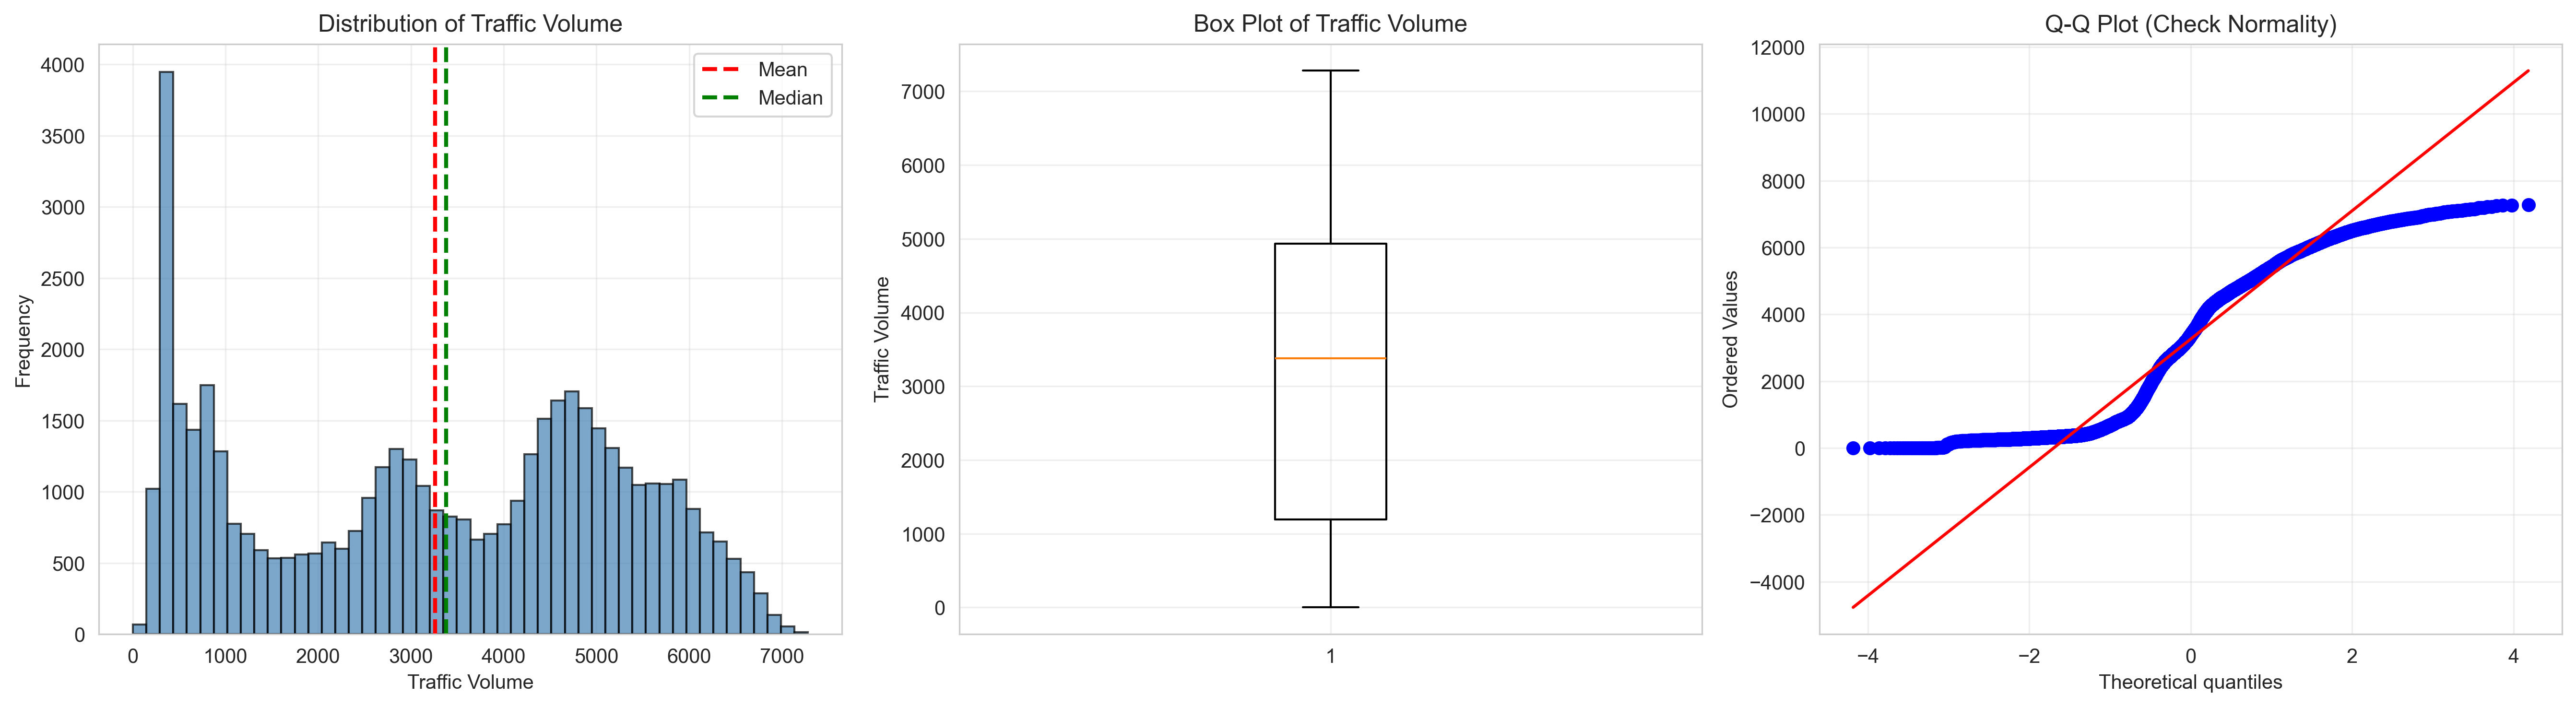
\includegraphics[width=1\textwidth]{images/eda_target_distribution.png}
    \caption{Distribution of Traffic Volume}
    \label{fig:eda_target_distribution}
\end{figure}

Secondly, I did a numeric feature analysis and created distribution histograms for all numeric features (4), Pearson correlation analysis with the target,
correlation visualization, and scatter plots with trend lines for the top correlated features.
It seems the distributions of temperature, rain, and snow are are tightly clustered while the clouds feature is more spreado out.
\begin{figure}[H]
    \centering
    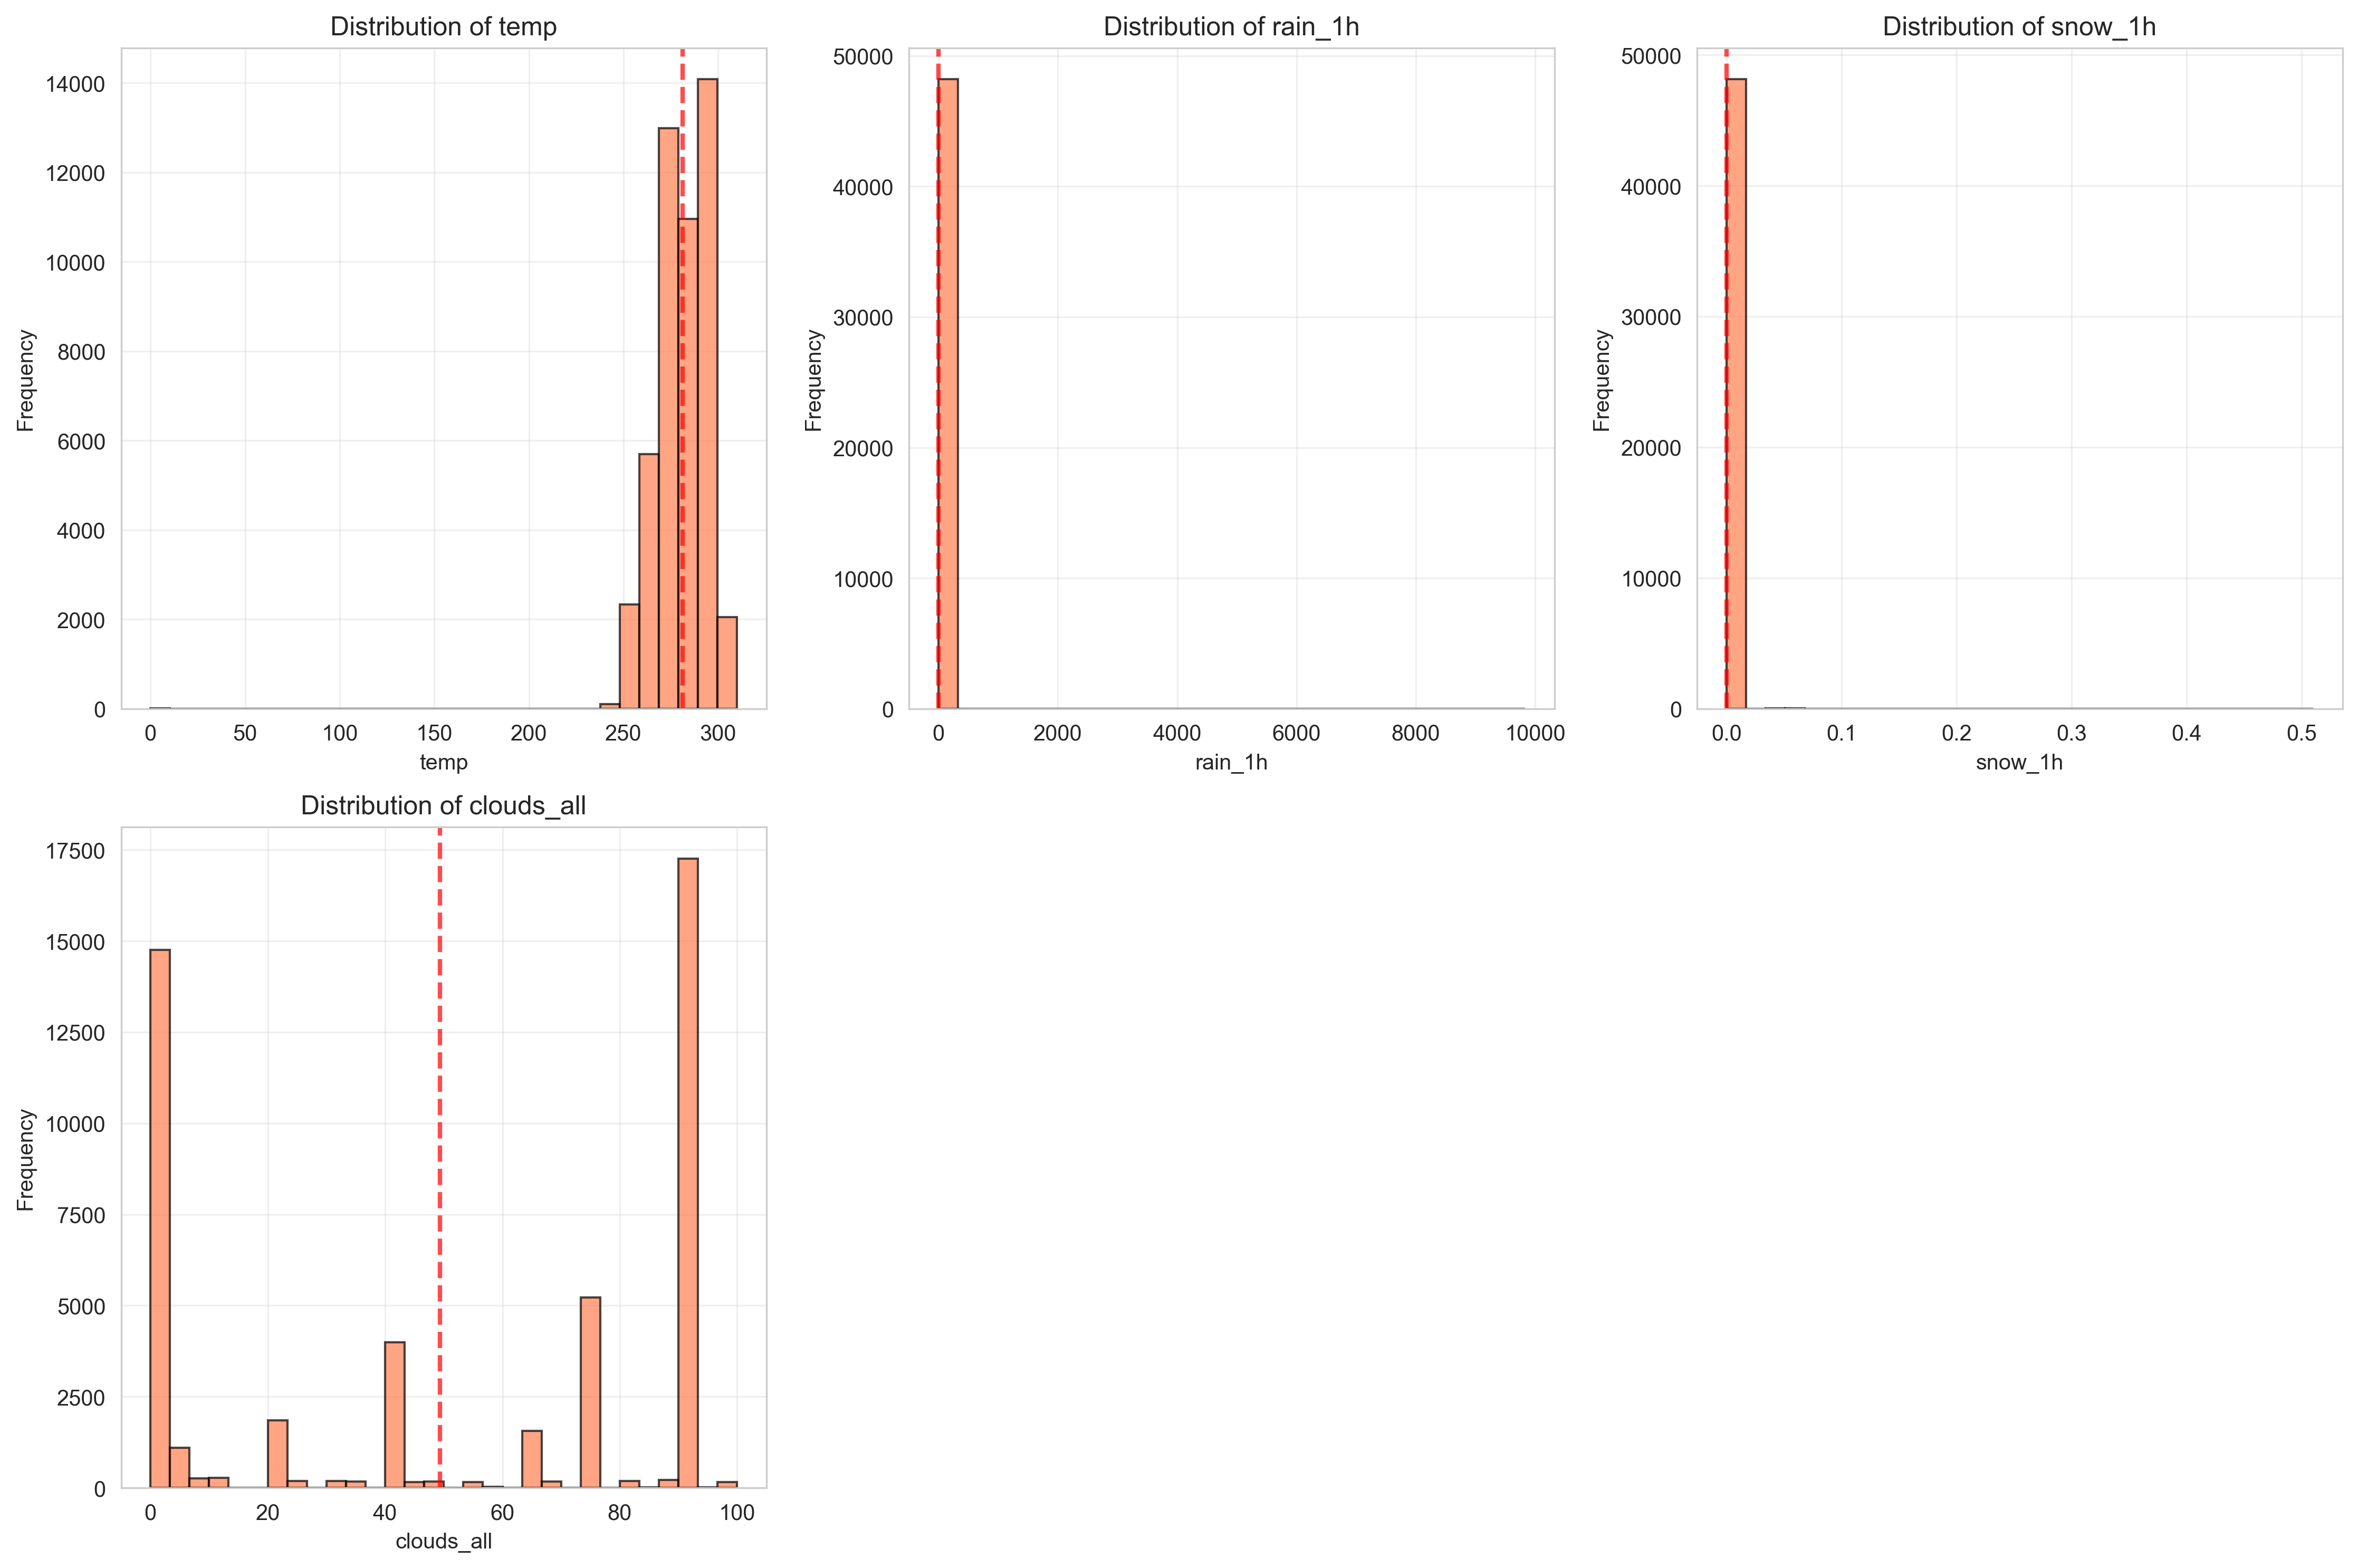
\includegraphics[width=1\textwidth]{images/eda_numeric_distributions.png}
    \caption{Distribution of Numeric Features}
    \label{fig:eda_numeric_distributions}
\end{figure}

It also appears that the temperature best correlates with traffic volume, showing a weak positive correlation of 0.130. This suggests that as temperature increases, 
there is a slight tendency for traffic volume to increase as well, possibly due to more people traveling in warmer weather.
\begin{figure}[H]
    \centering
    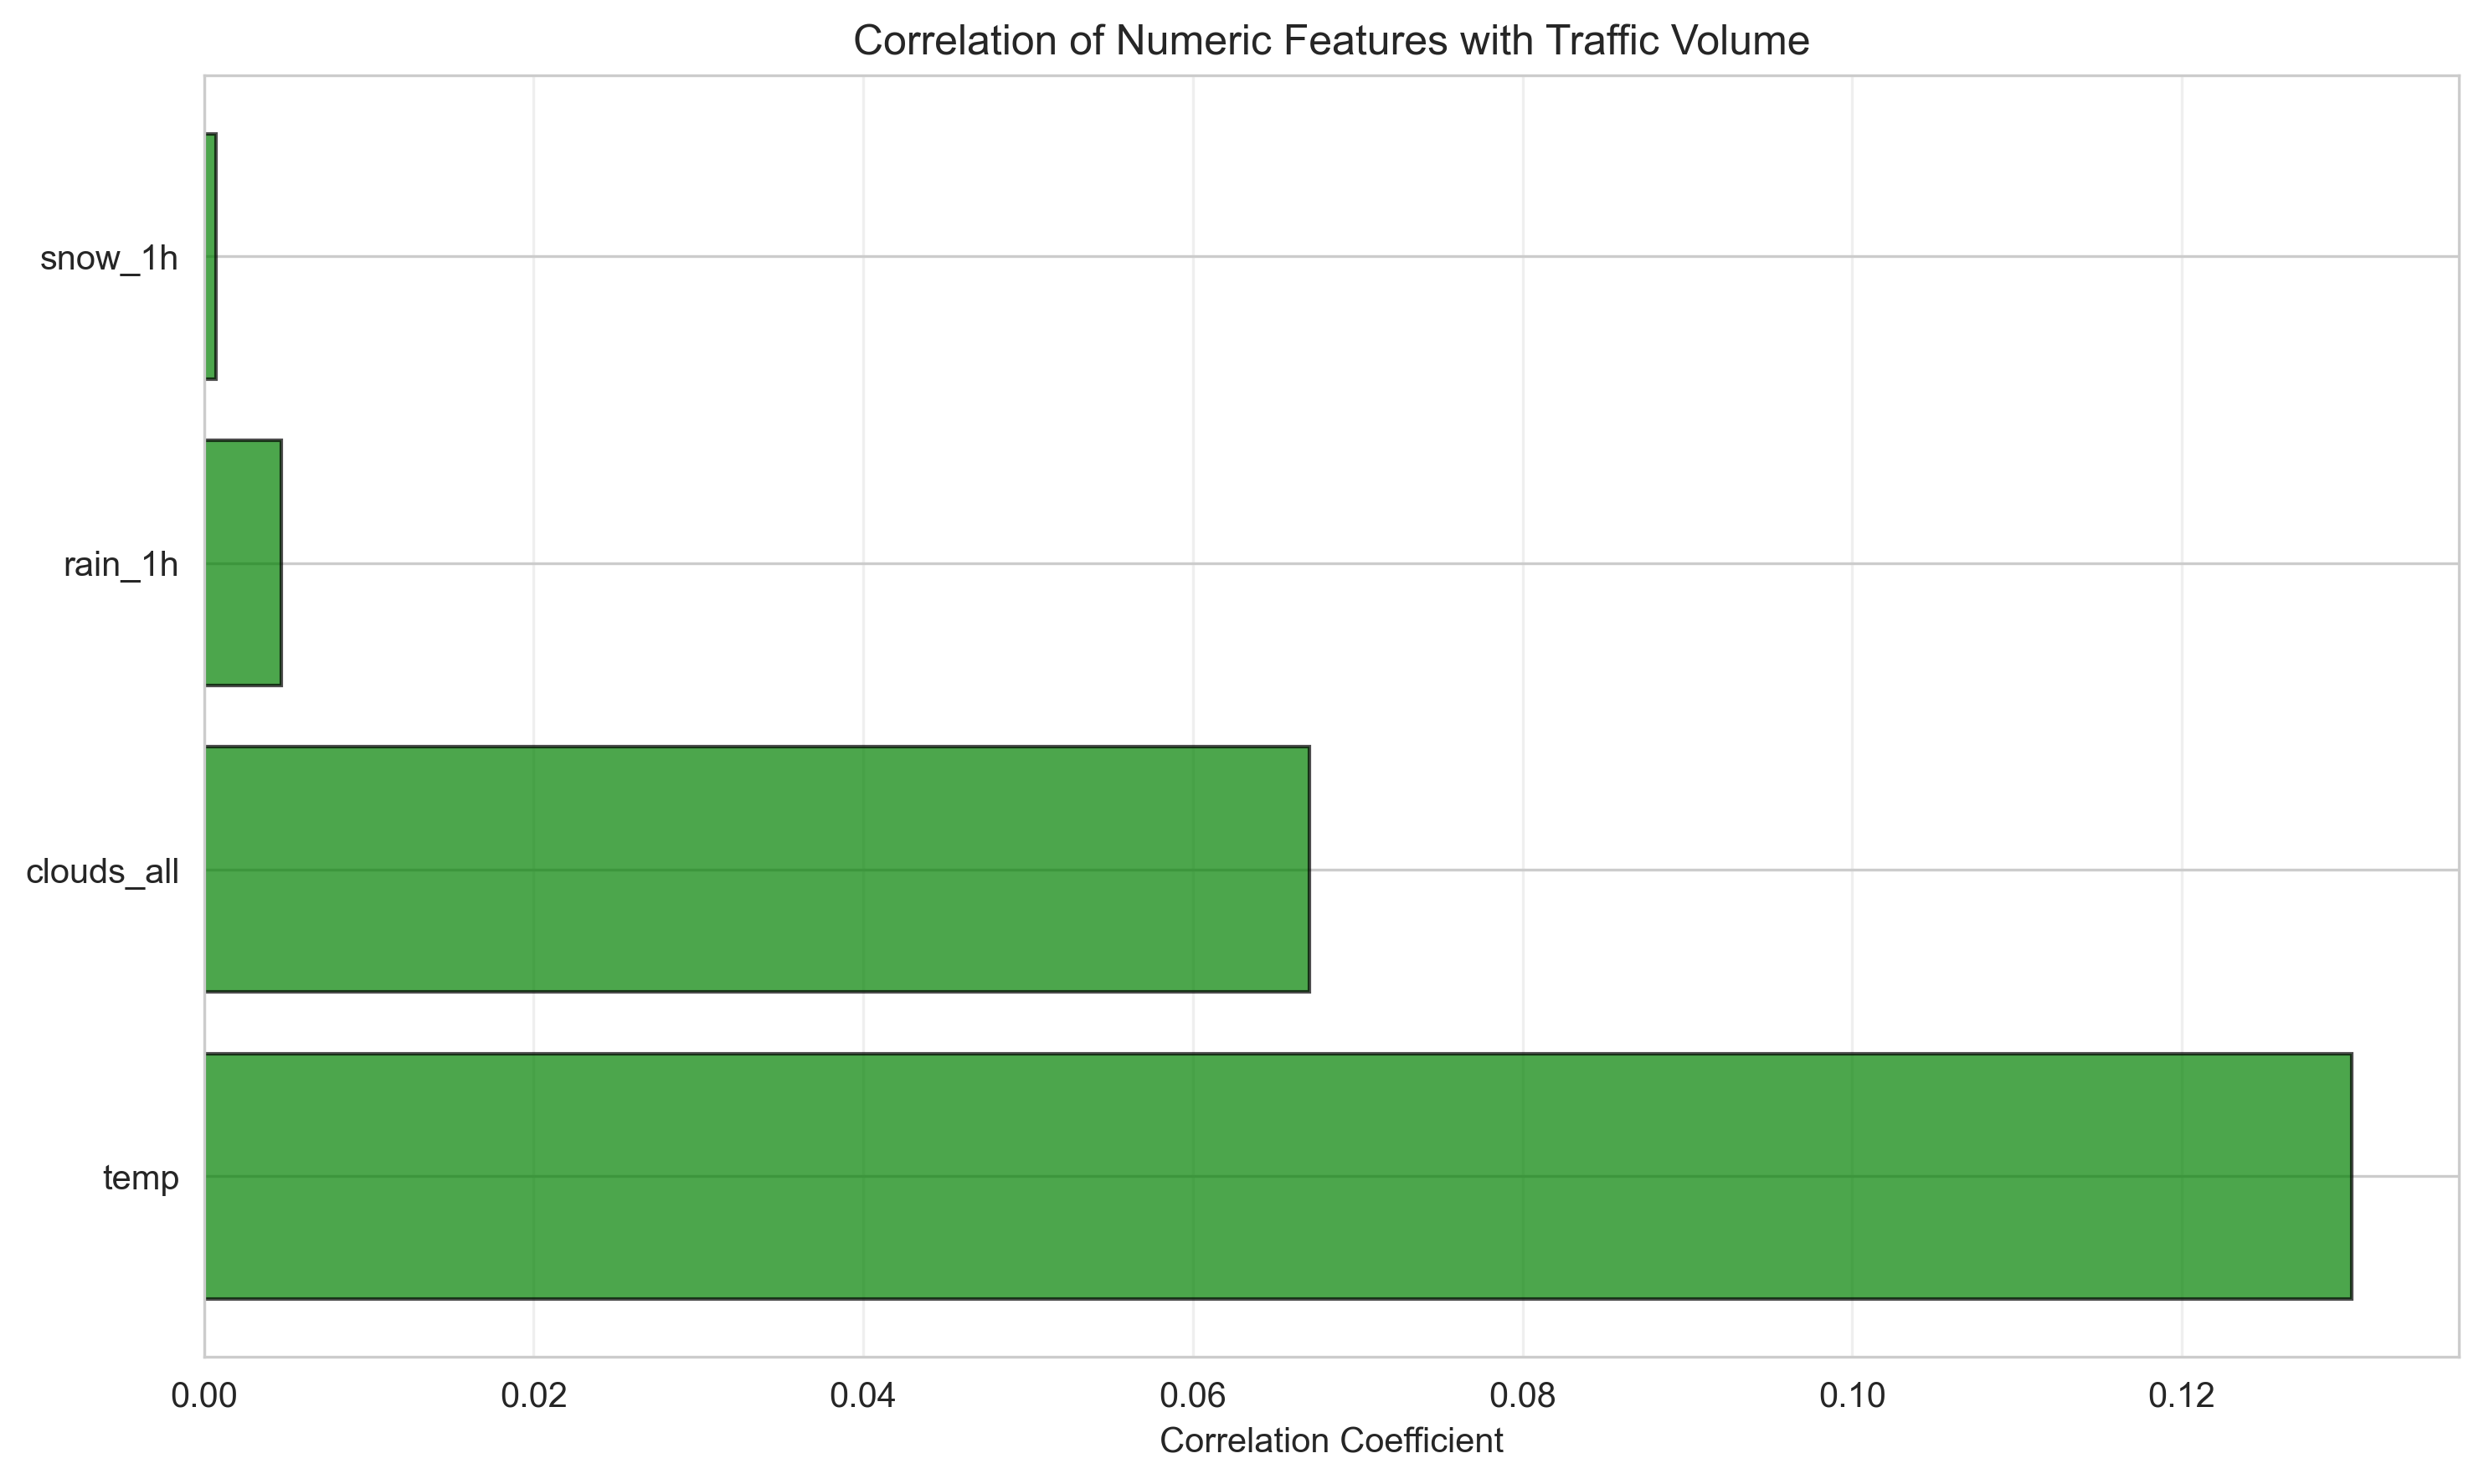
\includegraphics[width=1\textwidth]{images/eda_numeric_correlations.png}
    \caption{Numeric Feature Correlations with Traffic Volume}
    \label{fig:eda_numeric_correlations}
\end{figure}

Finally, the scatterplots don't provide strong evidence of linear relationships, but there is a slight upward trend between clouds and traffic volume.
\begin{figure}[H]
    \centering
    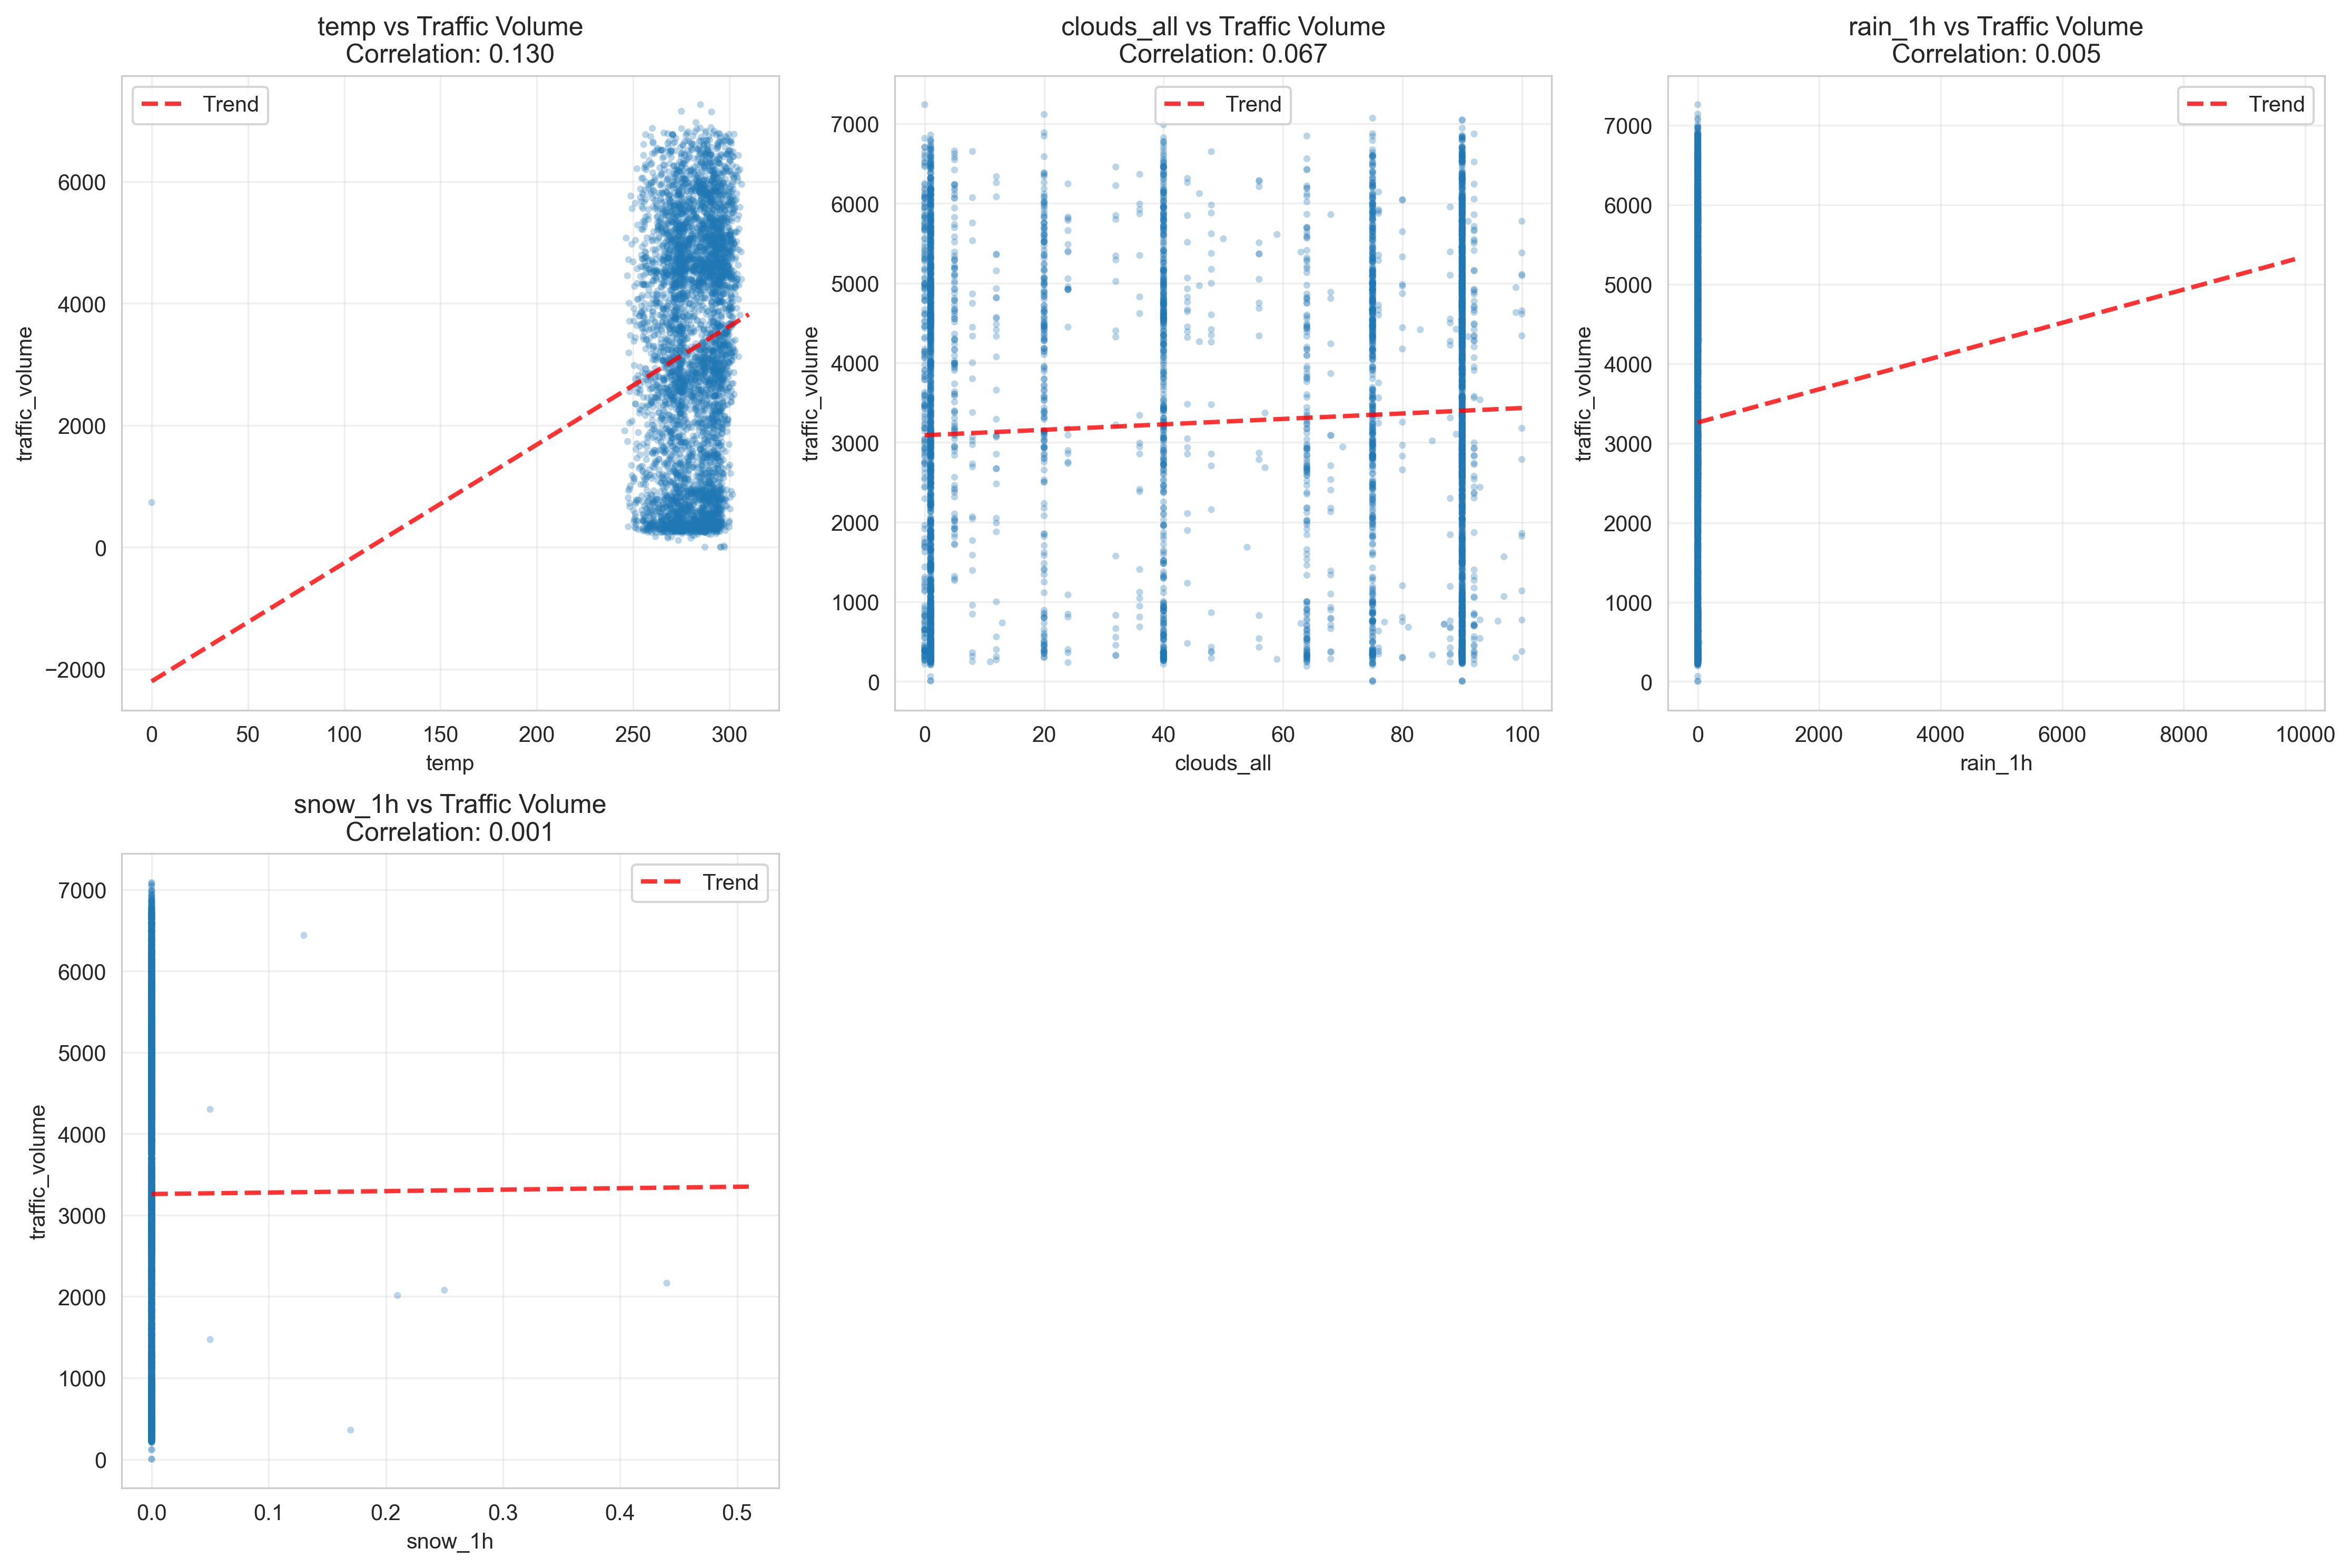
\includegraphics[width=1\textwidth]{images/eda_scatter_plots.png}
    \caption{Scatterplots of Top Numeric Features vs. Traffic Volume}
    \label{fig:eda_numeric_scatterplots}
\end{figure}

Then, I did an analysis on the categorical features (5). I created a distribution of counts of different classes in the categorical features,
and then analyzed the categorical features against the target variable using box plots and ANOVA tests to see if there were significant differences in traffic volume.

The distribution of the holiday feature shows that the vast majority of data points are non-holidays, and for the most part the holidays are evenly distributed which makes sense given the time frame the data was collected over.
For weather main and weather description, there are heavy skews towards clouds and sky is clear respectively. This indicates that most data was collected during clear weather conditions and that traffic volume will more than likely
be higher during these times. 

\begin{figure}[H]
    \centering
    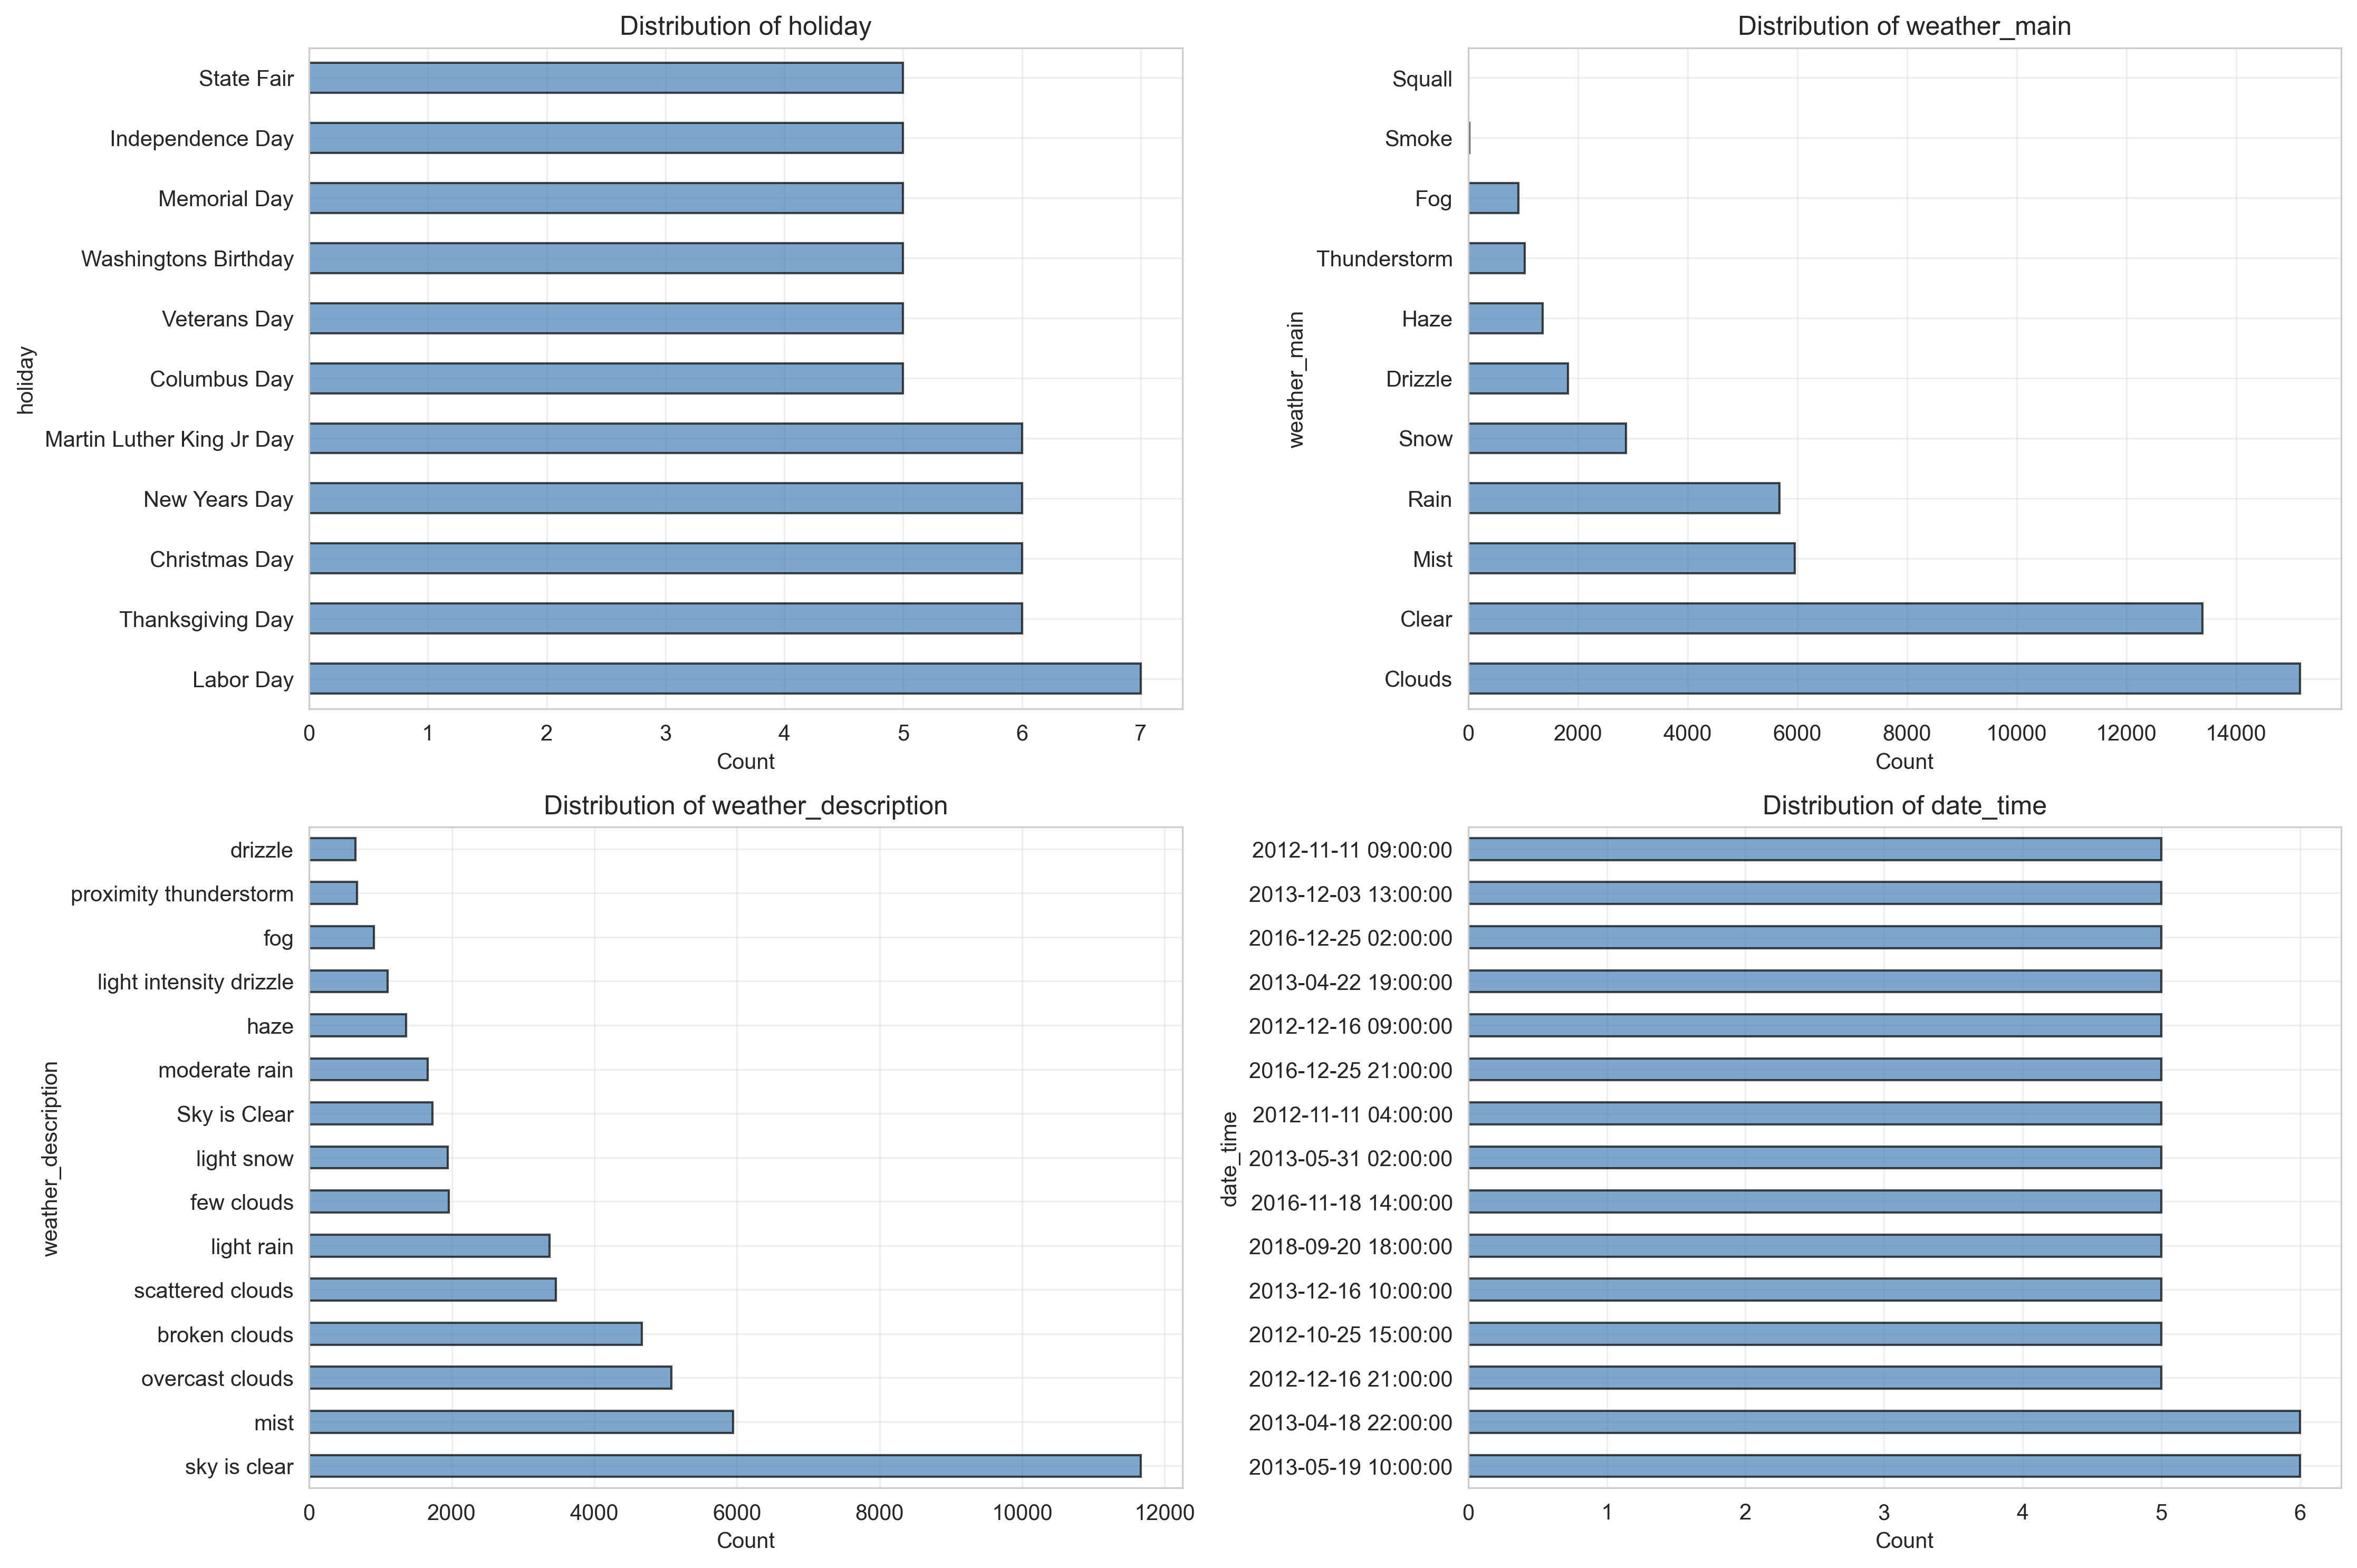
\includegraphics[width=1\textwidth]{images/eda_categorical_distributions.png}
    \caption{Distribution of Categorical Features}
    \label{fig:eda_categorical_distributions}
\end{figure}

Next, I created box plots to visualize the relationship between categorical features and traffic volume. The features weather main and weather description were bested boxplotted against
traffic volume and showed that traffic volume was highest during cloudy weather conditions. This goes against the idea (I just had) that the majority of traffic volume would be during "sky is clear" conditions.

\begin{figure}[H]
    \centering
    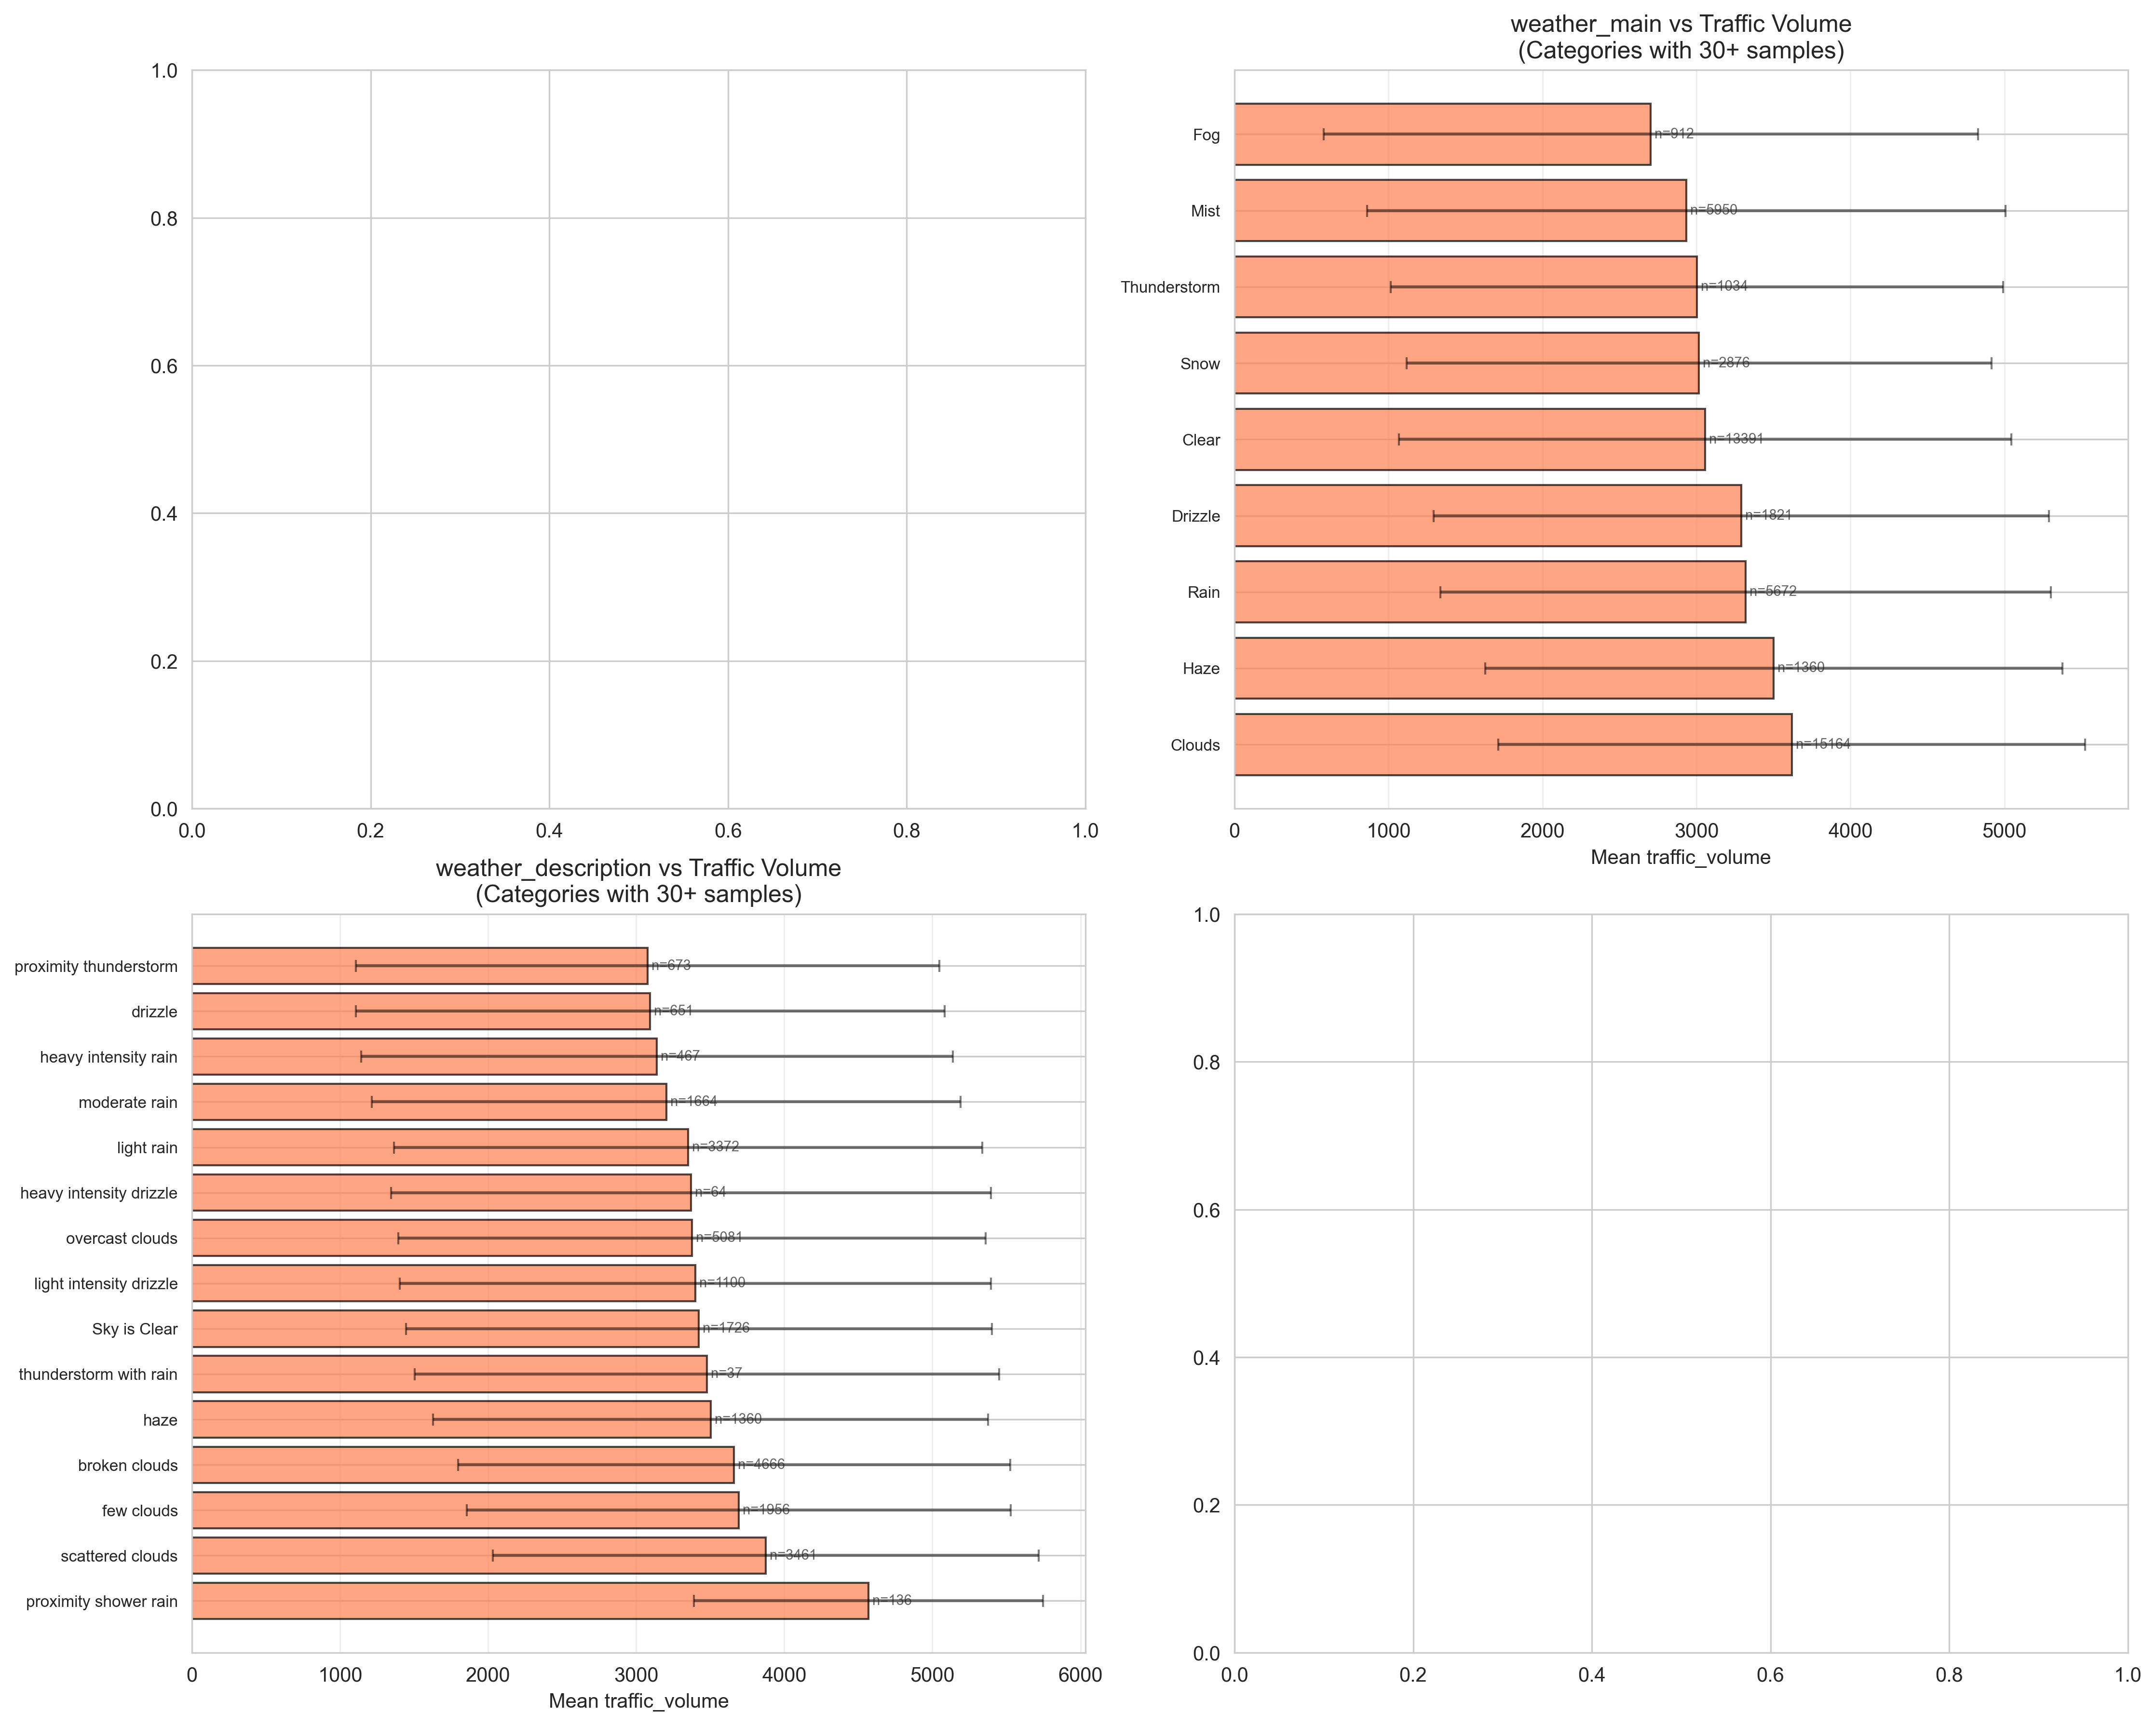
\includegraphics[width=1\textwidth]{images/eda_categorical_vs_target.png}
    \caption{Box Plots of Categorical Features vs. Traffic Volume}
    \label{fig:eda_categorical_boxplots}
\end{figure}

Finally, I performed ANOVA tests to statistically assess whether the mean traffic volumes differ significantly across the categories of each categorical feature.
The ANOVA results indicated that for features like weather main and weather description, they would be very predictive of traffic volume. This make sense when looking at the full picture because
when you are driving anywhere in bad conditions, people tend to slow down, drive more cautiously, or crash and cause traffic jams. So, the weather will be very important for prediction!

\subsection{3 ML Models}

I created three ML regressors (Linear Regression, Random Forest, XGBoost). I encoded hours cycically using sine and cosine transformations to capture the periodic nature of time. I encoded 
some binary features like "is\_weekend" and "is\_rush\_hour\_morning" as well for more interpretability. I then ended up with 42 features and fed them into the regressors and got these results:
\begin{lstlisting}
    LINEAR REGRESSION
    $R^2$ Score: 0.7841
    RMSE: 914.2879
    MAE: 706.4301
\end{lstlisting}

\begin{lstlisting}
    RANDOM FOREST REGRESSOR
    $R^2$ Score: 0.9405
    RMSE: 480.1658
    MAE: 279.2226
\end{lstlisting}

\begin{lstlisting}
    XGBOOST REGRESSOR
    $R^2$ Score: 0.9509
    RMSE: 436.1264
    MAE: 256.4578
\end{lstlisting}

\subsection{3 ML Models (with binning)}

Then, after creating categorical target by binning the volume into 3 different classes (Low, Medium, High), I created three classification models (Logistic Regression, Random Forest, XGBoost) and got these results:
\begin{lstlisting}
    LOGISTIC REGRESSION
Accuracy: 0.7764

Classification Report:
              precision    recall  f1-score   support

         Low       0.86      0.82      0.84      3183
      Medium       0.68      0.67      0.68      3310
        High       0.79      0.85      0.82      3148

    accuracy                           0.78      9641
   macro avg       0.78      0.78      0.78      9641
weighted avg       0.78      0.78      0.78      9641
\end{lstlisting}

\begin{lstlisting}
    RANDOM FOREST CLASSIFIER
Accuracy: 0.8956

Classification Report:
              precision    recall  f1-score   support

         Low       0.96      0.93      0.94      3183
      Medium       0.87      0.84      0.85      3310
        High       0.86      0.93      0.89      3148

    accuracy                           0.90      9641
   macro avg       0.90      0.90      0.90      9641
weighted avg       0.90      0.90      0.90      9641

    \end{lstlisting}

\begin{lstlisting}
    XGBOOST CLASSIFIER
Accuracy: 0.9018

Classification Report:
              precision    recall  f1-score   support

         Low       0.96      0.92      0.94      3183
      Medium       0.87      0.85      0.86      3310
        High       0.87      0.94      0.90      3148

    accuracy                           0.90      9641
   macro avg       0.90      0.90      0.90      9641
weighted avg       0.90      0.90      0.90      9641
\end{lstlisting}

And created some visualizations to compare the regression models and classification models.

\begin{figure}[H]
    \centering
    \includegraphics[width=1\textwidth]{images/regression_results.png}
    \caption{Regression Model Comparison}
    \label{fig:regression_comparison}
\end{figure}
\begin{figure}[H]
    \centering
    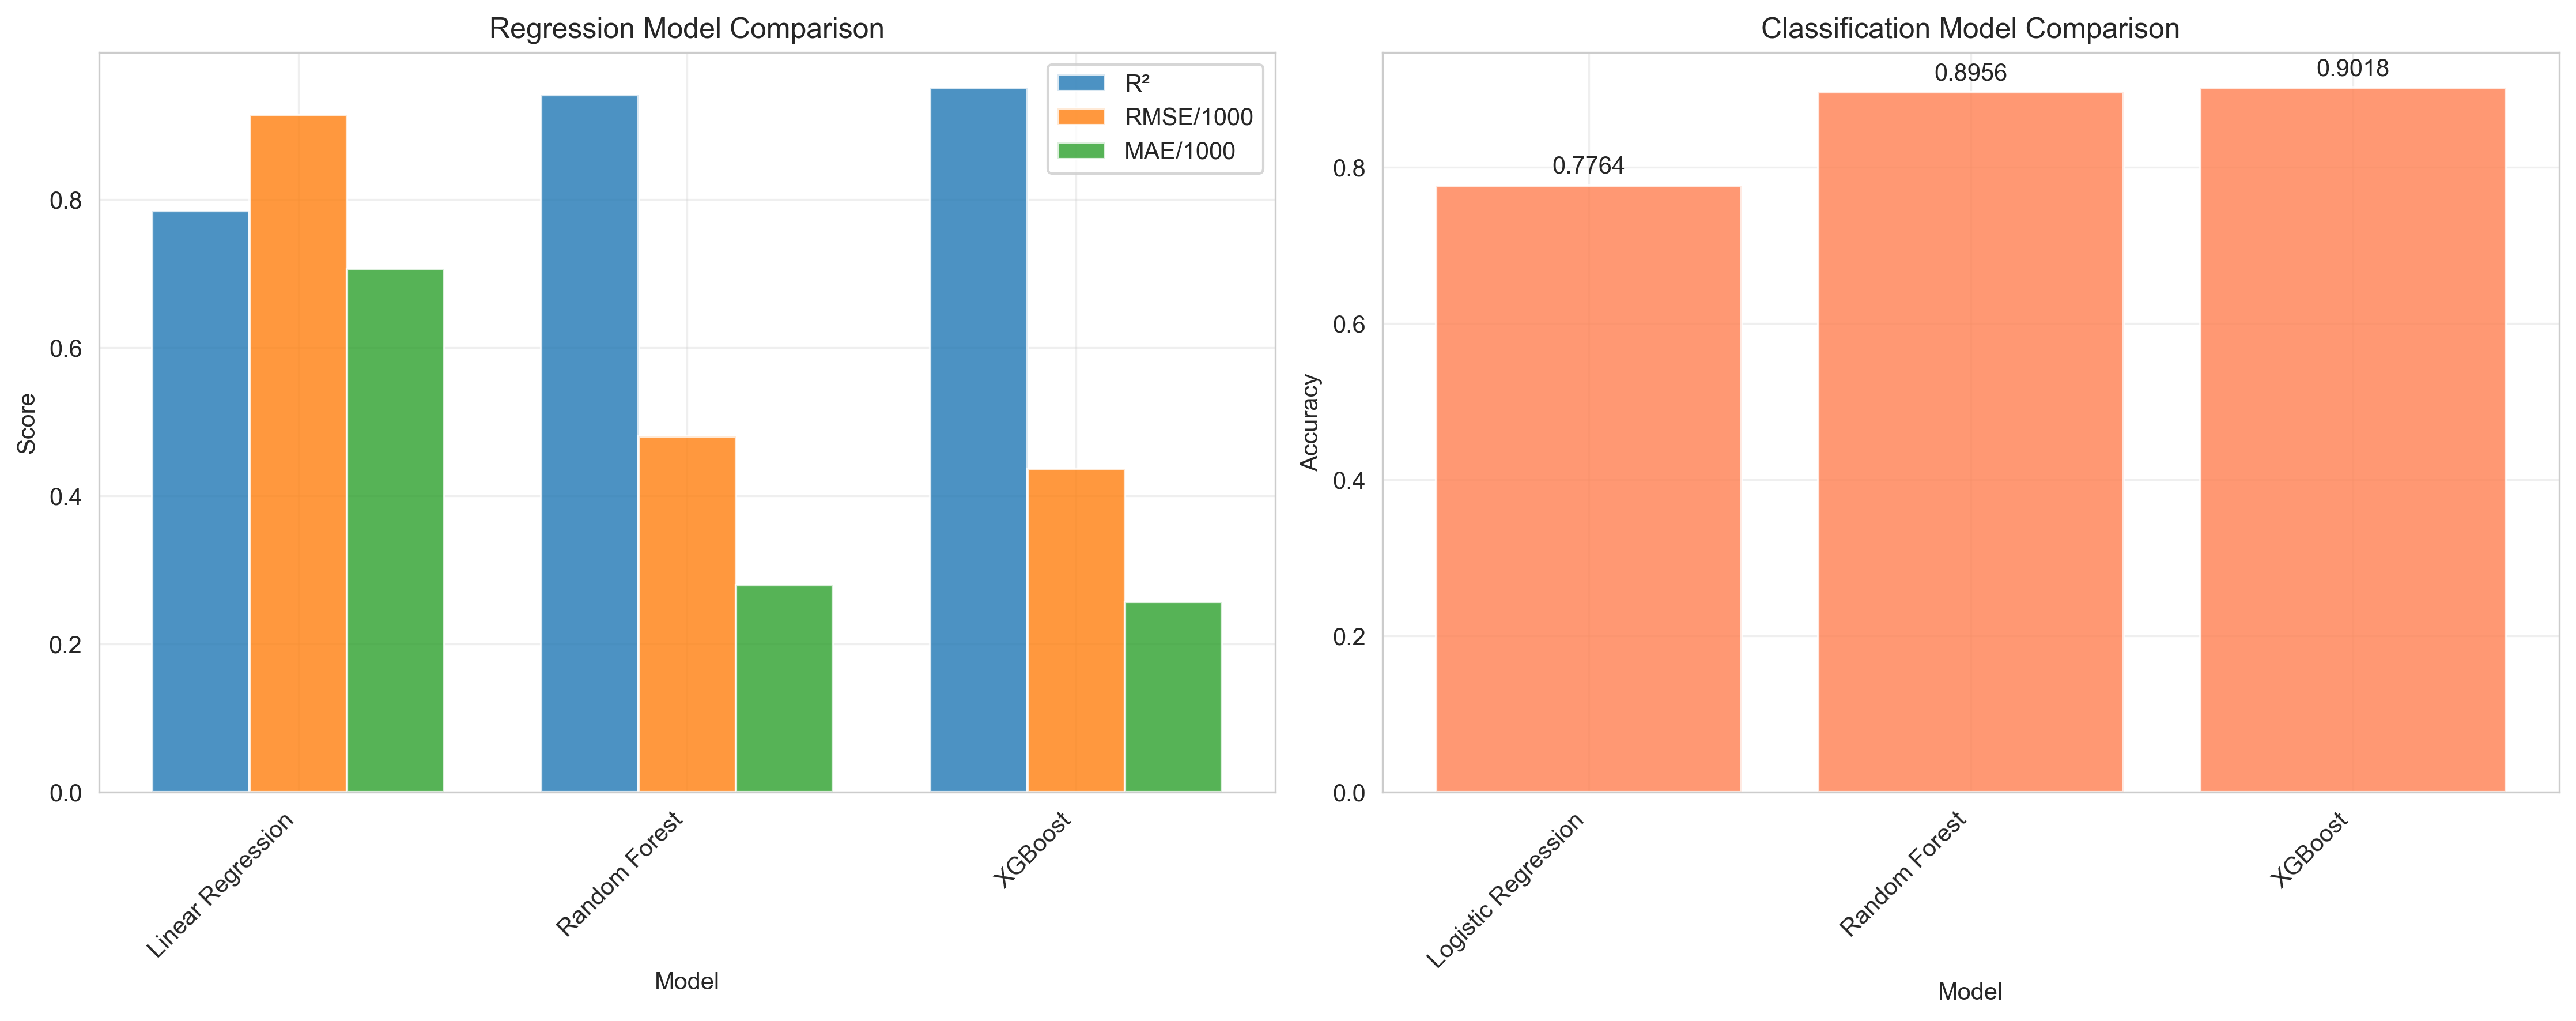
\includegraphics[width=1\textwidth]{images/model_comparison.png}
    \caption{Classification Model Comparison}
    \label{fig:classification_comparison}
\end{figure}
\begin{figure}
    \centering
    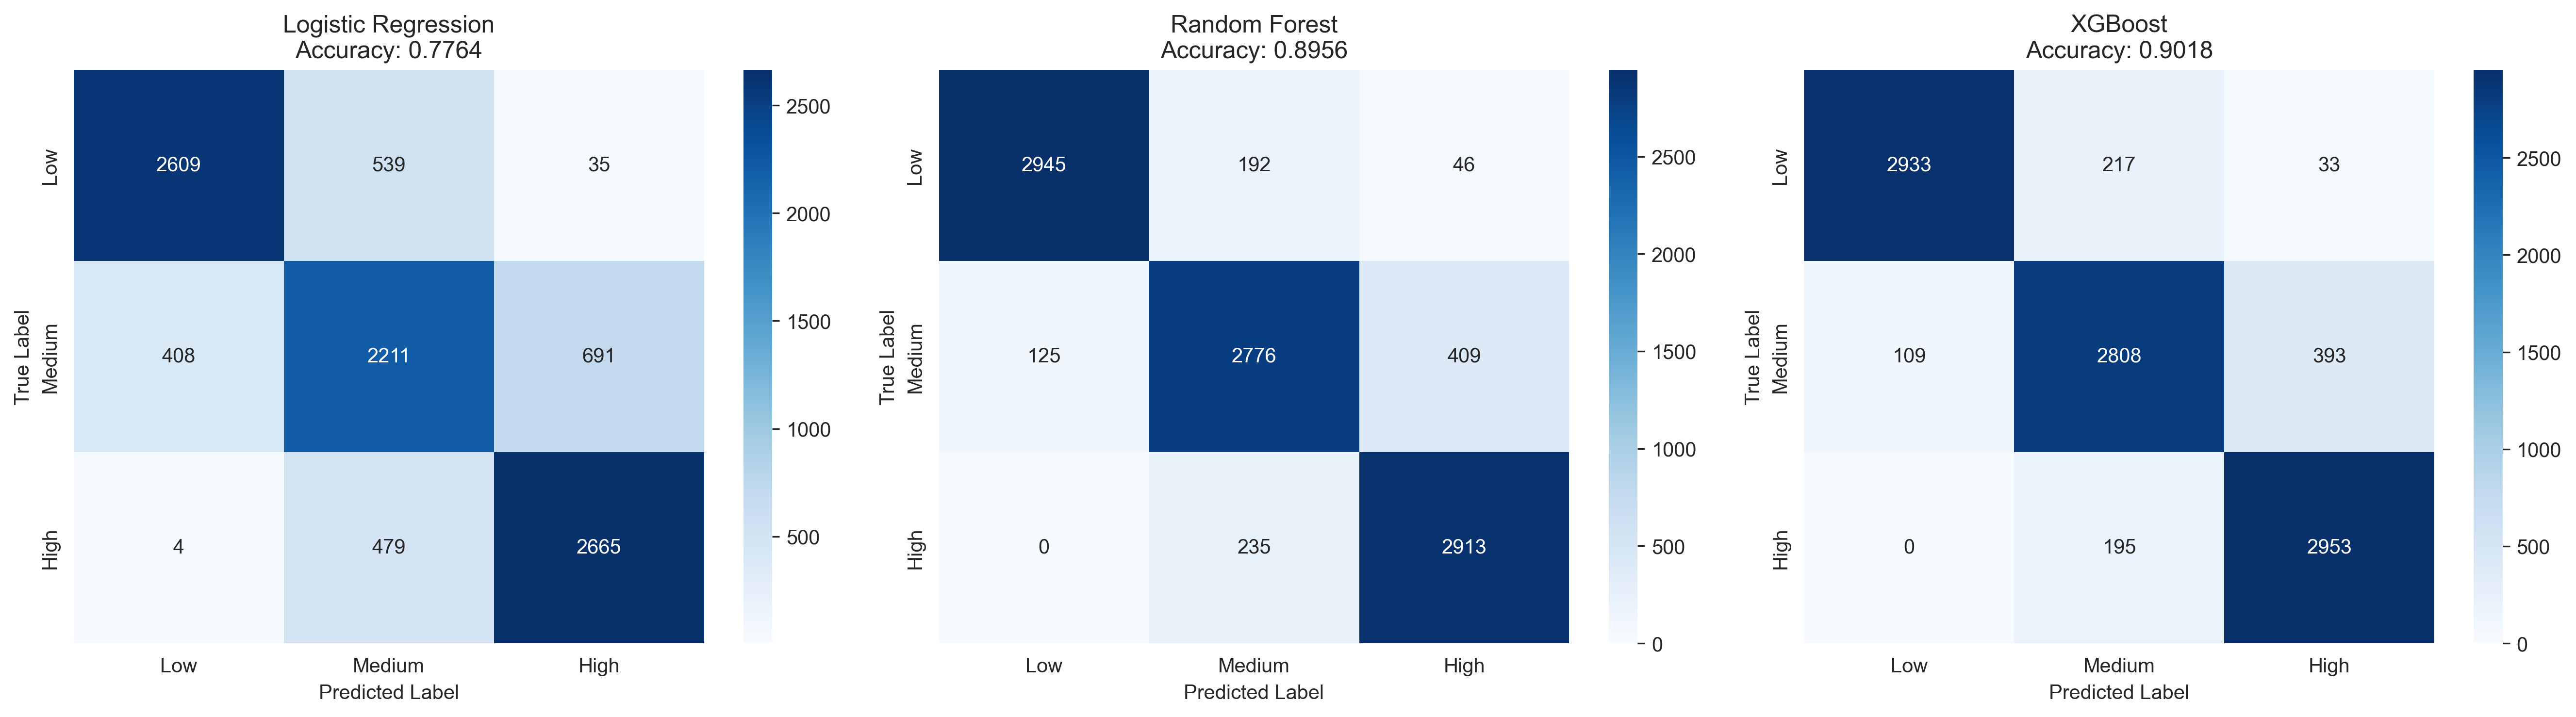
\includegraphics[width=1\textwidth]{images/confusion_matrices.png}
    \caption{Feature Importance from XGBoost Regressor}
    \label{fig:feature_importance}
\end{figure}
\begin{figure}
    \centering
    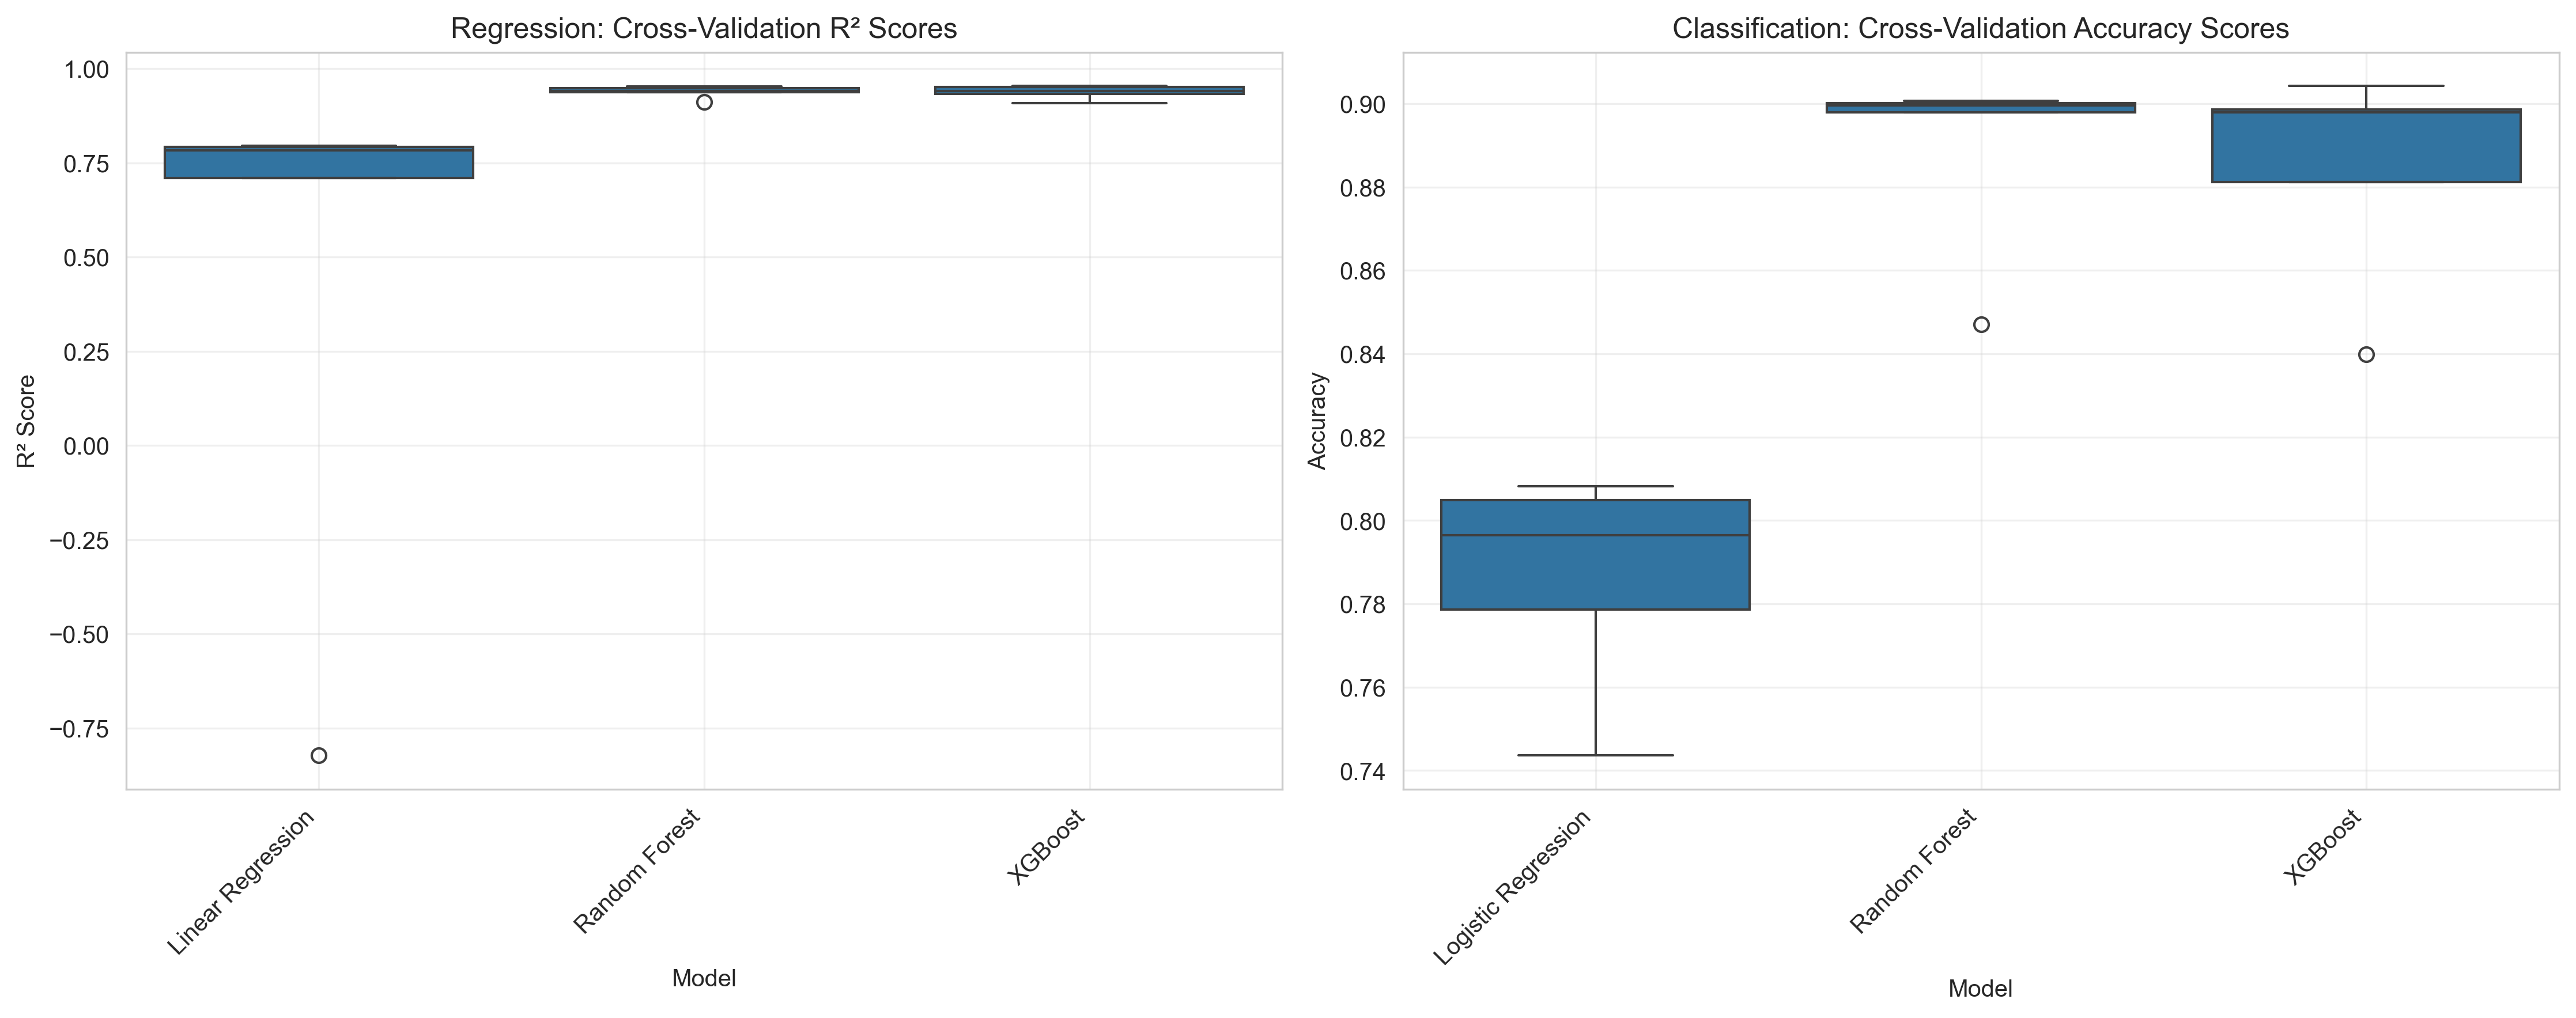
\includegraphics[width=1\textwidth]{images/cross_validation_comparison.png}
    \caption{Classification Model Confusion Matrices}
    \label{fig:classification_confusion_matrices}
\end{figure}

So, which methods work well?

\textbf{Regression:}
\begin{itemize}
    \item Tree-based models (Random Forest, XGBoost) typically outperform Linear Regression
    \item XGBoost often achieves the highest $R^2$ due to its gradient boosting and regularization
    \item Linear Regression struggles with non-linear temporal patterns and interactions
\end{itemize}

\textbf{Classification:}
\begin{itemize}
    \item All models typically achieve high accuracy (>70\%) due to clear separability
    \item Random Forest and XGBoost show more balanced performance across classes
    \item Logistic Regression may struggle with boundary cases between Medium/High
\end{itemize}

Those findings are nice and all, but what do we actually *do* with them? 

Some actionable insights: Regression is more actionable because it provides exact traffic volume predictions for capacity planning,
resource allocation (e.g., tolling, road maintenance), and trend analysis. 
Classification is more robust because it is less sensitive to outliers, easier to communicate, and more stable for alert systems.

So, while classification provides more robust predictions, regression offers more granular, actionable insights for urban traffic management.

However, what actions do we should we take based on these findings?

For operational planning (next hour/day predictions), regression models like XGBoost are best due to their high R² and low RMSE, allowing precise volume estimates.

For alert systems (traffic level warnings), classification models like Random Forest provide balanced precision/recall across classes, enabling reliable alerts without excessive false alarms.

For strategic planning (long-term capacity), regression models can analyze trends by aggregating predictions to daily/weekly/monthly averages, aiding resource budgeting.

The final verdict is that the best regression model is XGBoost with it's staggering R² of 0.9509, and the best classification model is Random Forest with its balanced accuracy of 89.56\%.
If we wanted to make reasonable and effective change using any of these models, it would be best to use the XGBoost regression for traffic volume predictions, with Random Forest classification as a backup/alert system.

\section{Code}

Here is a link to the Jupyter Notebook containing all code used for data exploration, model training, evaluation, and visualization: \href{https://colab.research.google.com/drive/1BKRMXI40PGC_hTNV45E3-m17CC6Ntb2-?usp=sharing}{The Code}.

\end{document}
